\section{Iterators}
\subsection{What they are}
\begin{frame}
  \frametitle{What is an Iterator?}
  \begin{block}{Design pattern [GoF]}
    Provide a way to access the elements of an aggregate object sequentially without exposing its underlying representation.
  \end{block}
  \vfill
  \begin{block}{Stepanov}
    Iterator is a coordinate.
  \end{block}
  \vfill
  \begin{block}{A generalization of a pointer}
    \begin{itemize}
    \item indirect access (\texttt{operator*()}, \texttt{operator->()})
    \item operations for moving to point to a new element (\texttt{operator++()}, \texttt{operator--()}) 
    \end{itemize}
  \end{block}
\end{frame}

\subsection{Iterators in the STL}

\begin{frame}
  \frametitle{Iterators in the STL}
  \begin{block}{Their role}
    \begin{itemize}
    \item Iterators are the glue that ties the standard-library alogorithms to their data
    \item Iterators are the mechanism used to minimize an algorithm's dependence on the data structures on which it operates.
      \end{itemize}
  \end{block}
\vfill
  \begin{block}{Alex Stepanov}
    The reason that STL containers and algorithms work so well together is that they know nothing of each other.
    \end{block}
\end{frame}

\begin{frame}[fragile]
  %% \frametitle{How to use iterators}
  \vfill
  \begin{lstlisting}
       while( first != last )
  \end{lstlisting}
  \vfill
\end{frame}


\subsection{Iterator categories}
\begin{frame}
  \frametitle{Iterator categories}
  \centering
  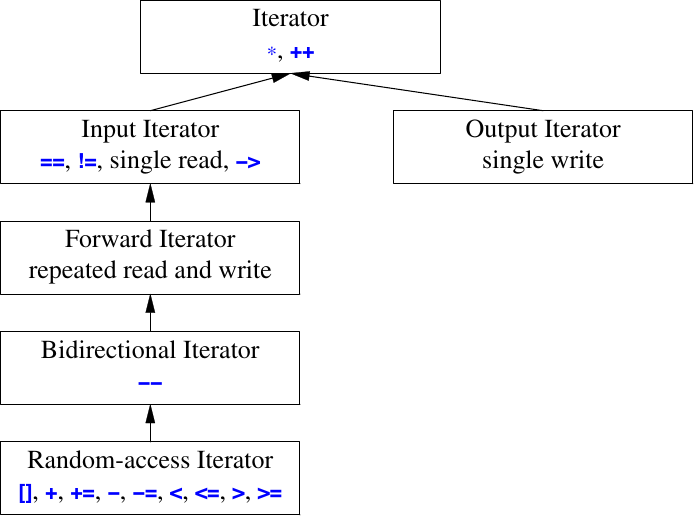
\includegraphics[height=0.8\textheight]{img/iterators.png}
\end{frame}

\begin{frame}[fragile]
  \frametitle{How to implement our own iterator?}
\begin{lstlisting}
  template <typename T>
  class List<T>::Iterator {
    ...
  };
\end{lstlisting}
\end{frame}

\subsection{Our List iterator}
\begin{frame}[fragile]
  \frametitle{How to implement our own iterator?}
\begin{lstlisting}
  #include <iterator>
  ...
  template <typename T>
  class List<T>::Iterator{
    typename List<T>::node* current;
    public:
    using value_type = T;
    using difference_type = std::ptrdiff_t;
    using iterator_category =
      std::forward_iterator_tag;
    using reference = value_type&;
    using pointer = value_type*;
    ...
\end{lstlisting}
\end{frame}

\begin{frame}[fragile]
  \frametitle{How to implement our own iterator?}
\begin{lstlisting}
    ...
    reference operator*() {
      return current->value; }
    pointer operator->() { return &**this; }
    Iterator& operator++() {
      current = current->next;
      return *this;
    }
    friend
    bool operator==(const Iterator&, const Iterator&);
    friend
    bool operator!=(const Iterator&, const Iterator&);
  };
\end{lstlisting}
\end{frame}

